\documentclass[../mathNotesPreamble]{subfiles}
\begin{document}
%\relscale{1.4} %TODO
\section{15.7: Maximum/Minimum Problems}
  \begin{ex*}
    Consider the function $f(x)=x^3-3x+1$ on the interval $\sbrkt{-1,2}$. Find the local extrema and absolute extrema of this function.
  \end{ex*}
  \vspace*{\stretch{1}}

  \begin{defn*}[Local Maximum/Minimum Values]
    Suppose $(a,b)$ is a point in a region $R$ on which $f$ is defined. 
    \begin{itemize}
      \item 
        If $f(x,y)\leq f(a,b)$ for all $(x,y)$ in the domain of $f$ and in some open disk centered at $(a,b)$, then $f(a,b)$ is a \textbf{local maximum value} of $f$.
      \item 
        If $f(x,y)\geq f(a,b)$ for all $(x,y)$ in the domain of $f$ and in some open disk centered at $(a,b)$, then $f(a,b)$ is a \textbf{local minimum value} of $f$.
      \item 
        Local maximum and local minimum values are also called \textbf{local extreme values} or \textbf{local extrema}.
    \end{itemize}
  \end{defn*}
  \pagebreak

  \begin{thmBox*}[Theorem 15.14: Derivatives and Local Maximum/Minimum Values]
    If $f$ has a local maximum or minimum value at $(a,b)$ and the partial derivatives $f_x$ and $f_y$ exist at $(a,b)$, then $f_x(a,b)=f_y(a,b)=0$.
  \end{thmBox*}

  \begin{defn*}[Critical Point]
    An interior point $(a,b)$ in the domain of $f$ is a \textbf{critical point} of $f$ if either
    \begin{enumerate}
      \item 
        $f_x(a,b)=f_y(a,b)=0$, or
      \item 
        at least one of the partial derivatives $f_x$ and $f_y$ does not exist at $(a,b)$.
    \end{enumerate}
  \end{defn*}

  \begin{ex*}
    Find the critical points of $f(x,y)=3(x-1)^2+4(2-y)^3$.
  \end{ex*}
  \vspace*{\stretch{1}}

  \begin{ex*}
    Find the critical points of $g(x,y)=x^2+xy-y^2$.
  \end{ex*}
  \vspace*{\stretch{1}}

  \begin{ex*}
    Find the critical points of $\ds h(x,y)=\frac{3}{x}-\frac{4}{y}$.
  \end{ex*}
  \vspace*{\stretch{1}}

  \pagebreak

  \begin{defn*}[Saddle Point]
    Consider a function $f$ that is differentiable at a critical point $(a,b)$. Then $f$ has a \textbf{saddle point} at $(a,b)$ if, in every open disk centered at $(a,b)$, there are points $(x,y)$ for which $f(x,y)>f(a,b)$ and points for which $f(x,y)<f(a,b)$.
  \end{defn*}

  \noindent
  \begin{minipage}[t]{0.65\linewidth}
    \begin{ex*}
      Compute the first and second order partial derivatives of $f(x,y)=x^2-y^2$.
    \end{ex*}
  \end{minipage}%
  \begin{minipage}[t]{0.35\linewidth}\mbox{}
    \begin{flushright}
      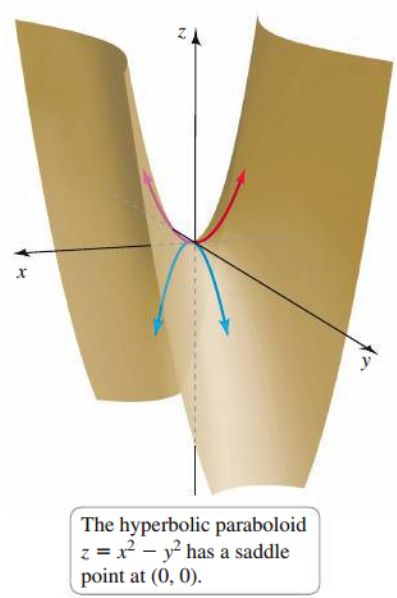
\includegraphics[width=0.8\linewidth]{../images/briggs_15_07/fig15_68}
    \end{flushright}
  \end{minipage}

  \begin{thmBox*}[Theorem 15.15: Second Derivative Test]
    Suppose the second partial derivatives of $f$ are continuous throughout an open disk centered at the point $(a,b)$, where $f_x(a,b)=f_y(a,b)=0$. Let 
      \[D(x,y)=f_{xx}(x,y) f_{yy}(x,y)-\parens{f_{xy}(x,y)}^2.\]
    \begin{enumerate}
      \item 
        If $D(a,b) > 0$ and $f_{xx}(a,b) < 0$, then $f$ has a local maximum value at $(a,b)$.
      \item 
        If $D(a,b) > 0$ and $f_{xx}(a,b) > 0$, then $f$ has a local minimum value at $(a,b)$.
      \item 
        If $D(a,b) <0$, then $f$ has a saddle point at $(a,b)$.
      \item 
        If $D(a,b)=0$, then the test is inconclusive.
    \end{enumerate}
  \end{thmBox*}
  \pagebreak

  \begin{ex*}
    Use the Second Derivative Test to classify the critical points of \newline
    $f(x,y)=x^2+2y^2-4x+4y+6$.
  \end{ex*}
  \vspace*{\stretch{1}}

  \begin{ex*}
    Use the Second Derivative Test to classify the critical points of \newline
    $f(x,y)=xy(x-2)(y+3)$.
  \end{ex*}
  \vspace*{\stretch{1}}
  \pagebreak

  \vspace*{\stretch{1}}
  \begin{defn*}[Absolute Maximum/Minimum Values]
    Let $f$ be defined on a set $R$ in $\bbr^2$ containing the point $(a,b)$. 
    \begin{itemize}
      \item 
        If $f(a,b)\geq f(x,y)$ for every $(x,y)$ in $R$, then $f(a,b)$ is an \textbf{absolute maximum value} of $f$ on $R$.
      \item 
        If $f(a,b)\leq f(x,y)$ for every $(x,y)$ in $R$, then $f(a,b)$ is an \textbf{absolute minimum value} of $f$ on $R$.
    \end{itemize}
  \end{defn*}
  \vspace*{\stretch{1}}
  \begin{thmBox*}[Procedure:\\ Finding Absolute Maximum/Minimum Values on Closed Bounded Sets]
    Let $f$ be continuous on a closed bounded set $R$ in $\bbr^2$. To find the absolute maximum and minimum values of $f$ on $R$:
    \begin{enumerate}
      \item 
        Determine the values of $f$ at all critical points in $R$.
      \item 
        Find the maximum and minimum values of $f$ on the boundary of $R$.
      \item 
        The greatest function value found in Steps 1 and 2 is the absolute maximum value of $f$ on $R$, and the least function value found in Steps 1 and 2 is the absolute minimum value of $f$ on $R$.
    \end{enumerate}
  \end{thmBox*}
  \vspace*{\stretch{1}}
  \pagebreak

  \begin{ex*}
    Find the absolute maximum and minimum values of $f(x,y)=xy-8x-y^2+12y+160$ over the triangular region $R=\set{(x,y): 0\leq x\leq 15,\ 0\leq y\leq 15-x}.$
  \end{ex*}
  \pagebreak

  \begin{ex*}
    A shipping company handles rectangular boxes provided the sum of the length, width, and height of the box does not exceed $96$ in. Find the dimensions of the box that meets this condition and has the largest volume.
  \end{ex*}
  \begin{flushright}
    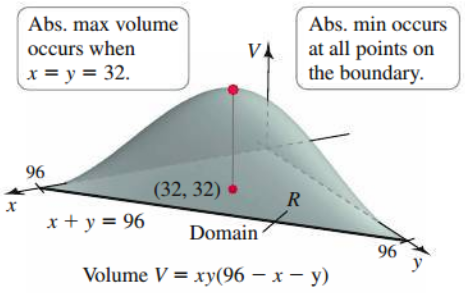
\includegraphics[width=0.4\linewidth]{../images/briggs_15_07/fig15_73}
  \end{flushright}
  \pagebreak

  \begin{ex*}
    Find the absolute maximum and minimum values of $f(x,y)=4-x^2-y^2$ on the open disk $R=\set{(x,y): x^2+y^2<1}$ (if they exist).
  \end{ex*}
  \pagebreak

  \begin{ex*}
    Find the point(s) on the plane $x+2y+z=2$ closest to the point $P(2,0,4)$.
  \end{ex*}
  \pagebreak
  
\end{document}